\documentclass[10pt,letterpaper]{article}

\usepackage[margin=0.75in]{geometry}
\usepackage{tikz}

\begin{document}

  \title{CS 321, Assignment 4}
  \author{Cody Malick\\
  \texttt{malickc@oregonstate.edu}}
  \date{\today}
  \maketitle

\section{}
This is an interesting problem. To get the answer, we need to construct an NFA,
reverse it, then construct a regex statement out of it. So, our initial NFA 
looks like this: \\

\begin{center}
	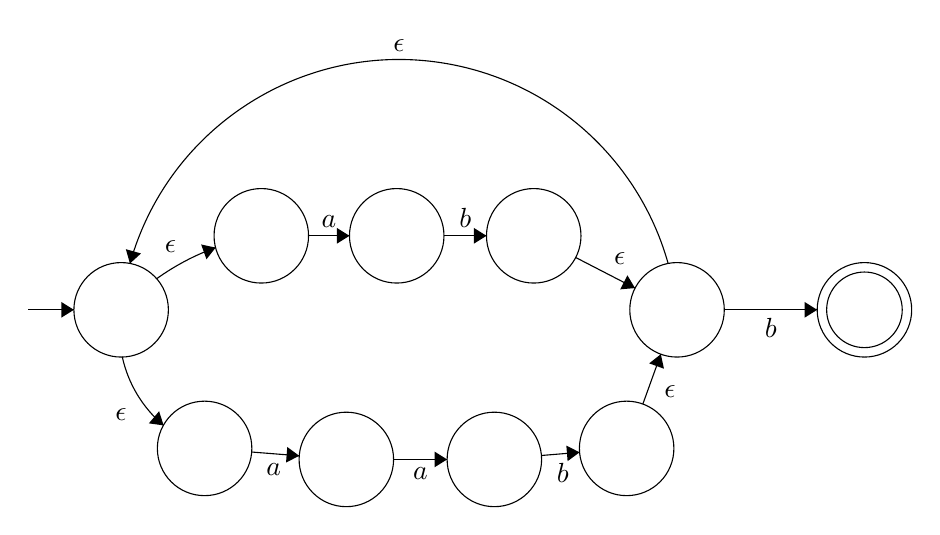
\begin{tikzpicture}[scale=0.2]
		\tikzstyle{every node}+=[inner sep=0pt]
		\draw [black] (7.2,-19.5) circle (3);
		\draw [black] (16.1,-14.8) circle (3);
		\draw [black] (42.5,-19.5) circle (3);
		\draw [black] (12.5,-28.3) circle (3);
		\draw [black] (54.4,-19.5) circle (3);
		\draw [black] (54.4,-19.5) circle (2.4);
		\draw [black] (24.7,-14.8) circle (3);
		\draw [black] (33.4,-14.8) circle (3);
		\draw [black] (21.5,-29) circle (3);
		\draw [black] (30.9,-29) circle (3);
		\draw [black] (39.3,-28.3) circle (3);
		\draw [black] (1.3,-19.5) -- (4.2,-19.5);
		\fill [black] (4.2,-19.5) -- (3.4,-19) -- (3.4,-20);
		\draw [black] (45.5,-19.5) -- (51.4,-19.5);
		\fill [black] (51.4,-19.5) -- (50.6,-19) -- (50.6,-20);
		\draw (48.45,-20) node [below] {$b$};
		\draw [black] (7.763,-16.557) arc (164.31971:15.68029:17.747);
		\fill [black] (7.76,-16.56) -- (8.46,-15.92) -- (7.5,-15.65);
		\draw (24.85,-3.11) node [above] {$\epsilon$};
		\draw [black] (9.898,-26.843) arc (-130.13525:-167.74593:7.898);
		\fill [black] (9.9,-26.84) -- (9.61,-25.94) -- (8.96,-26.71);
		\draw (7.58,-26.15) node [left] {$\epsilon$};
		\draw [black] (15.49,-28.53) -- (18.51,-28.77);
		\fill [black] (18.51,-28.77) -- (17.75,-28.21) -- (17.67,-29.2);
		\draw (16.89,-29.21) node [below] {$a$};
		\draw [black] (24.5,-29) -- (27.9,-29);
		\fill [black] (27.9,-29) -- (27.1,-28.5) -- (27.1,-29.5);
		\draw (26.2,-29.5) node [below] {$a$};
		\draw [black] (33.89,-28.75) -- (36.31,-28.55);
		\fill [black] (36.31,-28.55) -- (35.47,-28.12) -- (35.55,-29.11);
		\draw (35.24,-29.22) node [below] {$b$};
		\draw [black] (40.33,-25.48) -- (41.47,-22.32);
		\fill [black] (41.47,-22.32) -- (40.73,-22.9) -- (41.67,-23.24);
		\draw (41.66,-24.69) node [right] {$\epsilon$};
		\draw [black] (36.07,-16.18) -- (39.83,-18.12);
		\fill [black] (39.83,-18.12) -- (39.35,-17.31) -- (38.89,-18.2);
		\draw (38.86,-16.65) node [above] {$\epsilon$};
		\draw [black] (27.7,-14.8) -- (30.4,-14.8);
		\fill [black] (30.4,-14.8) -- (29.6,-14.3) -- (29.6,-15.3);
		\draw (29.05,-14.3) node [above] {$b$};
		\draw [black] (19.1,-14.8) -- (21.7,-14.8);
		\fill [black] (21.7,-14.8) -- (20.9,-14.3) -- (20.9,-15.3);
		\draw (20.4,-14.3) node [above] {$a$};
		\draw [black] (9.453,-17.527) arc (125.6763:109.99986:15.532);
		\fill [black] (13.2,-15.55) -- (12.28,-15.35) -- (12.62,-16.29);
		\draw (10.34,-15.91) node [above] {$\epsilon$};
	\end{tikzpicture}
\end{center}

Reverse the NFA: \\
\begin{center}
	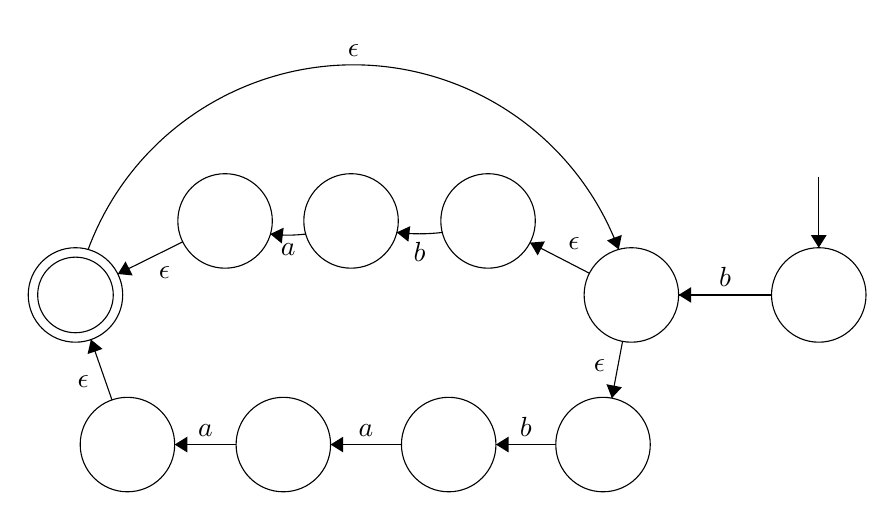
\begin{tikzpicture}[scale=0.2]
		\tikzstyle{every node}+=[inner sep=0pt]
		\draw [black] (7.2,-19.5) circle (3);
		\draw [black] (7.2,-19.5) circle (2.4);
		\draw [black] (16.7,-14.8) circle (3);
		\draw [black] (42.5,-19.5) circle (3);
		\draw [black] (10.5,-29) circle (3);
		\draw [black] (54.4,-19.5) circle (3);
		\draw [black] (24.7,-14.8) circle (3);
		\draw [black] (33.4,-14.8) circle (3);
		\draw [black] (20.4,-29) circle (3);
		\draw [black] (30.9,-29) circle (3);
		\draw [black] (40.7,-29) circle (3);
		\draw [black] (8.004,-16.613) arc (159.66022:20.33978:17.967);
		\fill [black] (41.7,-16.61) -- (41.89,-15.69) -- (40.95,-16.04);
		\draw (24.85,-4.39) node [above] {$\epsilon$};
		\draw [black] (41.94,-22.45) -- (41.26,-26.05);
		\fill [black] (41.26,-26.05) -- (41.9,-25.36) -- (40.92,-25.17);
		\draw (40.87,-23.96) node [left] {$\epsilon$};
		\draw [black] (39.83,-18.12) -- (36.07,-16.18);
		\fill [black] (36.07,-16.18) -- (36.55,-16.99) -- (37.01,-16.1);
		\draw (38.86,-16.65) node [above] {$\epsilon$};
		\draw [black] (30.498,-15.53) arc (-83.05694:-96.94306:11.98);
		\fill [black] (27.6,-15.53) -- (28.34,-16.12) -- (28.46,-15.13);
		\draw (29.05,-16.12) node [below] {$b$};
		\draw [black] (21.831,-15.633) arc (-83.02591:-96.97409:9.319);
		\fill [black] (19.57,-15.63) -- (20.3,-16.23) -- (20.42,-15.23);
		\draw (20.7,-16.2) node [below] {$a$};
		\draw [black] (14.01,-16.13) -- (9.89,-18.17);
		\fill [black] (9.89,-18.17) -- (10.83,-18.26) -- (10.38,-17.37);
		\draw (12.86,-17.65) node [below] {$\epsilon$};
		\draw [black] (37.7,-29) -- (33.9,-29);
		\fill [black] (33.9,-29) -- (34.7,-29.5) -- (34.7,-28.5);
		\draw (35.8,-28.5) node [above] {$b$};
		\draw [black] (27.9,-29) -- (23.4,-29);
		\fill [black] (23.4,-29) -- (24.2,-29.5) -- (24.2,-28.5);
		\draw (25.65,-28.5) node [above] {$a$};
		\draw [black] (17.4,-29) -- (13.5,-29);
		\fill [black] (13.5,-29) -- (14.3,-29.5) -- (14.3,-28.5);
		\draw (15.45,-28.5) node [above] {$a$};
		\draw [black] (9.52,-26.17) -- (8.18,-22.33);
		\fill [black] (8.18,-22.33) -- (7.97,-23.25) -- (8.92,-22.93);
		\draw (8.09,-24.99) node [left] {$\epsilon$};
		\draw [black] (54.4,-12) -- (54.4,-16.5);
		\fill [black] (54.4,-16.5) -- (54.9,-15.7) -- (53.9,-15.7);
		\draw [black] (51.4,-19.5) -- (45.5,-19.5);
		\fill [black] (45.5,-19.5) -- (46.3,-20) -- (46.3,-19);
		\draw (48.45,-19) node [above] {$b$};
	\end{tikzpicture}
\end{center}

And then tranlate that into a new regex statement:\\
\noindent $b(ba+baa)^*$
\section{}	
\begin{center}
	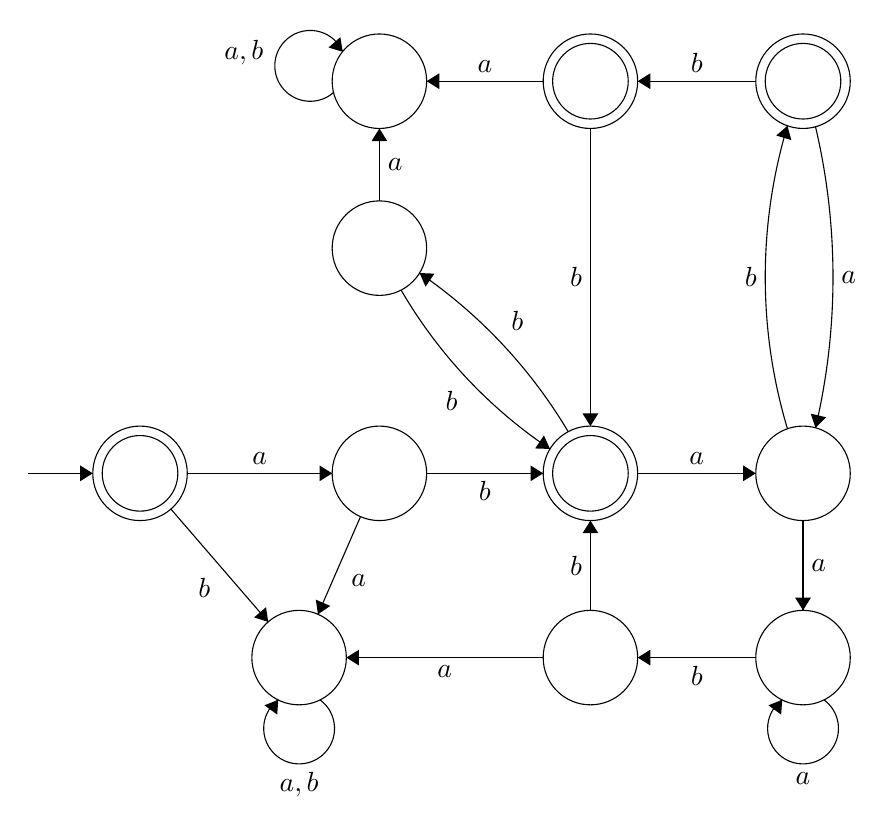
\begin{tikzpicture}[scale=0.2]
		\tikzstyle{every node}+=[inner sep=0pt]
		\draw [black] (10.9,-34.6) circle (3);
		\draw [black] (10.9,-34.6) circle (2.4);
		\draw [black] (26.1,-34.6) circle (3);
		\draw [black] (39.5,-34.6) circle (3);
		\draw [black] (39.5,-34.6) circle (2.4);
		\draw [black] (53,-34.6) circle (3);
		\draw [black] (53,-9.7) circle (3);
		\draw [black] (53,-9.7) circle (2.4);
		\draw [black] (53,-46.3) circle (3);
		\draw [black] (39.5,-46.3) circle (3);
		\draw [black] (21,-46.3) circle (3);
		\draw [black] (39.5,-9.7) circle (3);
		\draw [black] (39.5,-9.7) circle (2.4);
		\draw [black] (26.1,-9.7) circle (3);
		\draw [black] (26.1,-20.3) circle (3);
		\draw [black] (3.8,-34.6) -- (7.9,-34.6);
		\fill [black] (7.9,-34.6) -- (7.1,-34.1) -- (7.1,-35.1);
		\draw [black] (13.9,-34.6) -- (23.1,-34.6);
		\fill [black] (23.1,-34.6) -- (22.3,-34.1) -- (22.3,-35.1);
		\draw (18.5,-34.1) node [above] {$a$};
		\draw [black] (29.1,-34.6) -- (36.5,-34.6);
		\fill [black] (36.5,-34.6) -- (35.7,-34.1) -- (35.7,-35.1);
		\draw (32.8,-35.1) node [below] {$b$};
		\draw [black] (42.5,-34.6) -- (50,-34.6);
		\fill [black] (50,-34.6) -- (49.2,-34.1) -- (49.2,-35.1);
		\draw (46.25,-34.1) node [above] {$a$};
		\draw [black] (52.011,-31.769) arc (-163.30991:-196.69009:33.492);
		\fill [black] (52.01,-12.53) -- (51.3,-13.15) -- (52.26,-13.44);
		\draw (50.1,-22.15) node [left] {$b$};
		\draw [black] (53,-37.6) -- (53,-43.3);
		\fill [black] (53,-43.3) -- (53.5,-42.5) -- (52.5,-42.5);
		\draw (53.5,-40.45) node [right] {$a$};
		\draw [black] (50,-46.3) -- (42.5,-46.3);
		\fill [black] (42.5,-46.3) -- (43.3,-46.8) -- (43.3,-45.8);
		\draw (46.25,-46.8) node [below] {$b$};
		\draw [black] (39.5,-43.3) -- (39.5,-37.6);
		\fill [black] (39.5,-37.6) -- (39,-38.4) -- (40,-38.4);
		\draw (39,-40.45) node [left] {$b$};
		\draw [black] (36.5,-46.3) -- (24,-46.3);
		\fill [black] (24,-46.3) -- (24.8,-46.8) -- (24.8,-45.8);
		\draw (30.25,-46.8) node [below] {$a$};
		\draw [black] (22.323,-48.98) arc (54:-234:2.25);
		\draw (21,-53.55) node [below] {$a,b$};
		\fill [black] (19.68,-48.98) -- (18.8,-49.33) -- (19.61,-49.92);
		\draw [black] (12.86,-36.87) -- (19.04,-44.03);
		\fill [black] (19.04,-44.03) -- (18.9,-43.1) -- (18.14,-43.75);
		\draw (15.4,-41.9) node [left] {$b$};
		\draw [black] (24.9,-37.35) -- (22.2,-43.55);
		\fill [black] (22.2,-43.55) -- (22.98,-43.02) -- (22.06,-42.62);
		\draw (24.28,-41.42) node [right] {$a$};
		\draw [black] (54.323,-48.98) arc (54:-234:2.25);
		\draw (53,-53.55) node [below] {$a$};
		\fill [black] (51.68,-48.98) -- (50.8,-49.33) -- (51.61,-49.92);
		\draw [black] (50,-9.7) -- (42.5,-9.7);
		\fill [black] (42.5,-9.7) -- (43.3,-10.2) -- (43.3,-9.2);
		\draw (46.25,-9.2) node [above] {$b$};
		\draw [black] (36.5,-9.7) -- (29.1,-9.7);
		\fill [black] (29.1,-9.7) -- (29.9,-10.2) -- (29.9,-9.2);
		\draw (32.8,-9.2) node [above] {$a$};
		\draw [black] (23.197,-10.41) arc (311.47119:23.47119:2.25);
		\draw (18.76,-7.86) node [left] {$a,b$};
		\fill [black] (23.77,-7.83) -- (23.62,-6.9) -- (22.87,-7.56);
		\draw [black] (39.5,-12.7) -- (39.5,-31.6);
		\fill [black] (39.5,-31.6) -- (40,-30.8) -- (39,-30.8);
		\draw (39,-22.15) node [left] {$b$};
		\draw [black] (53.793,-12.593) arc (13.2596:-13.2596:41.669);
		\fill [black] (53.79,-31.71) -- (54.46,-31.04) -- (53.49,-30.81);
		\draw (55.4,-22.15) node [right] {$a$};
		\draw [black] (28.649,-21.88) arc (55.52835:30.74977:32.172);
		\fill [black] (28.65,-21.88) -- (29.03,-22.75) -- (29.59,-21.92);
		\draw (34.45,-24.94) node [right] {$b$};
		\draw [black] (36.932,-33.051) arc (-123.88325:-149.83864:30.782);
		\fill [black] (36.93,-33.05) -- (36.55,-32.19) -- (35.99,-33.02);
		\draw (31.1,-30.01) node [left] {$b$};
		\draw [black] (26.1,-17.3) -- (26.1,-12.7);
		\fill [black] (26.1,-12.7) -- (25.6,-13.5) -- (26.6,-13.5);
		\draw (26.6,-15) node [right] {$a$};
	\end{tikzpicture}
\end{center}
\section{}
To show that this DFA has at least 1024 states, we need to prove that having
less that 1024 states rejects a string in $A$, or show that there is a string
not in the language $A$ that the machine accepts. More specifically, we can
show that if machine $M$ has $<1024$ states, then feeding a string with $1024$
characters must prove there is a cycle, showing that it is regular.\\

This can be shown by accounting for every possible combination after the cycle
ends of alphabet $\{a,b\}^*$ leading up to the accepting state. This leaves us
with $2^{10}$ combinations. If we propose that the machine $M$ has less than 1024
states, then we can provide a string of length: number of states + 1, then we
can show there is a string that is rejected by $M$.

Given alphabet $A=\{a,b\}^*$, consider all strings of length 10, $w\in A$. Given
a string of length ten, there are two possible combinations for each position
in the string. Therefore, the total number of possible combinations of strings
are $2^{10}$.

Given that the number of states is less than 1024, then there must be a
combination in the alphabet $A$ that is not accepted. 

\section{}
Step 1:\\
Adversary picks $p$\\
Step 2:\\
I select $w=a^p b^p c^{p-p}$, where $|w|>=p$, and $w \in A$ and $w \in
$ real numbers\\
Step 3:\\
Split into $w=xyz$ where $|xy|=<p$, and $|y|>0$ \\
Step 4:\\
I pick $i=0$, I win if $xy^iz \notin A$\\
Then $xy^0z=xz=a^{p-|y|}c^0 \notin A$ since $|y|>0$\\
I win, A is not regular. 

\end{document}
